% !TEX root = ../FundationsDataScience.tex

\chapter{Convex Analysis}
\label{chap-convex-optim}

The main references for this chapter are \cite{ciarlet1982introduction,boyd2004convex}.
%
This chapters uses different notations than the previous one, and we denote $f(x)$ a typical function to minimized with respect to the variable $x$. 
%
We discus here some important concepts from convex analysis for non-smooth optimization. 


%%%%%%%%%%%%%%%%%%%%%%%%%%%%%%%%%%%%%%%%%%%%%%%%%%%%%%%%%%%%%%%%%%%%%%%%%%%%%%%%%%
%%%%%%%%%%%%%%%%%%%%%%%%%%%%%%%%%%%%%%%%%%%%%%%%%%%%%%%%%%%%%%%%%%%%%%%%%%%%%%%%%%
%%%%%%%%%%%%%%%%%%%%%%%%%%%%%%%%%%%%%%%%%%%%%%%%%%%%%%%%%%%%%%%%%%%%%%%%%%%%%%%%%%
\section{Basics of Convex Analysis}

We consider minimization problems of the form
\eql{\label{eq-convex-function}
	\umin{x \in \Hh} f(x)
}
over the finite dimension (Hilbertian) space $\Hh \eqdef \RR^N$, with the canonical inner product $\dotp{\cdot}{\cdot}$. 
%
Most of the results of this chapter extends to possibly infinite dimensional Hilbert space. 

Here $f : \Hh \longrightarrow \bar \RR \eqdef \RR \cup \{+\infty\}$ is a convex function. Note that we allow here $f$ to take the value $+\infty$ to integrate constraints in the objective, and the constraint set is thus the ``domain'' of the function
\eq{
	\dom(f) \eqdef \enscond{x}{f(x)<+\infty}.
}

A useful notation is the indicator function of a set $\Cc \subset \Hh$
\eq{
	\iota_{\Cc}(x) \eqdef \choice{
		0 \qifq x \in \Cc, \\
		+\infty \quad\text{otherwise.}
	}
}


%%%%%%%%%%%%%%%%%%%%%%%%%%%%%%%%%%%%%%%%%%%%%%%%%%%%%%%%%%%%%%%%%%%%%%%%%%%%%%%%%%
\subsection{Convex Sets and Functions}

A convex set $\Om \subset \Hh$ is such that
\eq{
	\foralls (x,y,t) \in \Hh^2 \times [0,1], \quad (1-t)x+ty \in \Om.
}
A convex function is such that 
\eql{\label{eq-convex-defn}
	\foralls (x,y,t) \in \Hh^2 \times [0,1], \quad f( (1-t)x+ty ) \leq (1-t)f(x) + t f(y)
}
and this is equivalent to its epigraph $\enscond{(x,r) \in \Hh \times \RR}{r \geq f(x)}$ being a convex set. Note that here we use $\leq$ as a comparison over $\bar\RR$. 
%
The function $f$ is strictly convex if equality in~\eqref{eq-convex-defn} only holds for $t \in \{0,1\}$.
%
A set $\Om$ being convex is equivalent to $\iota_{\Cc}$ being a convex function.



\begin{figure}
\centering
%%
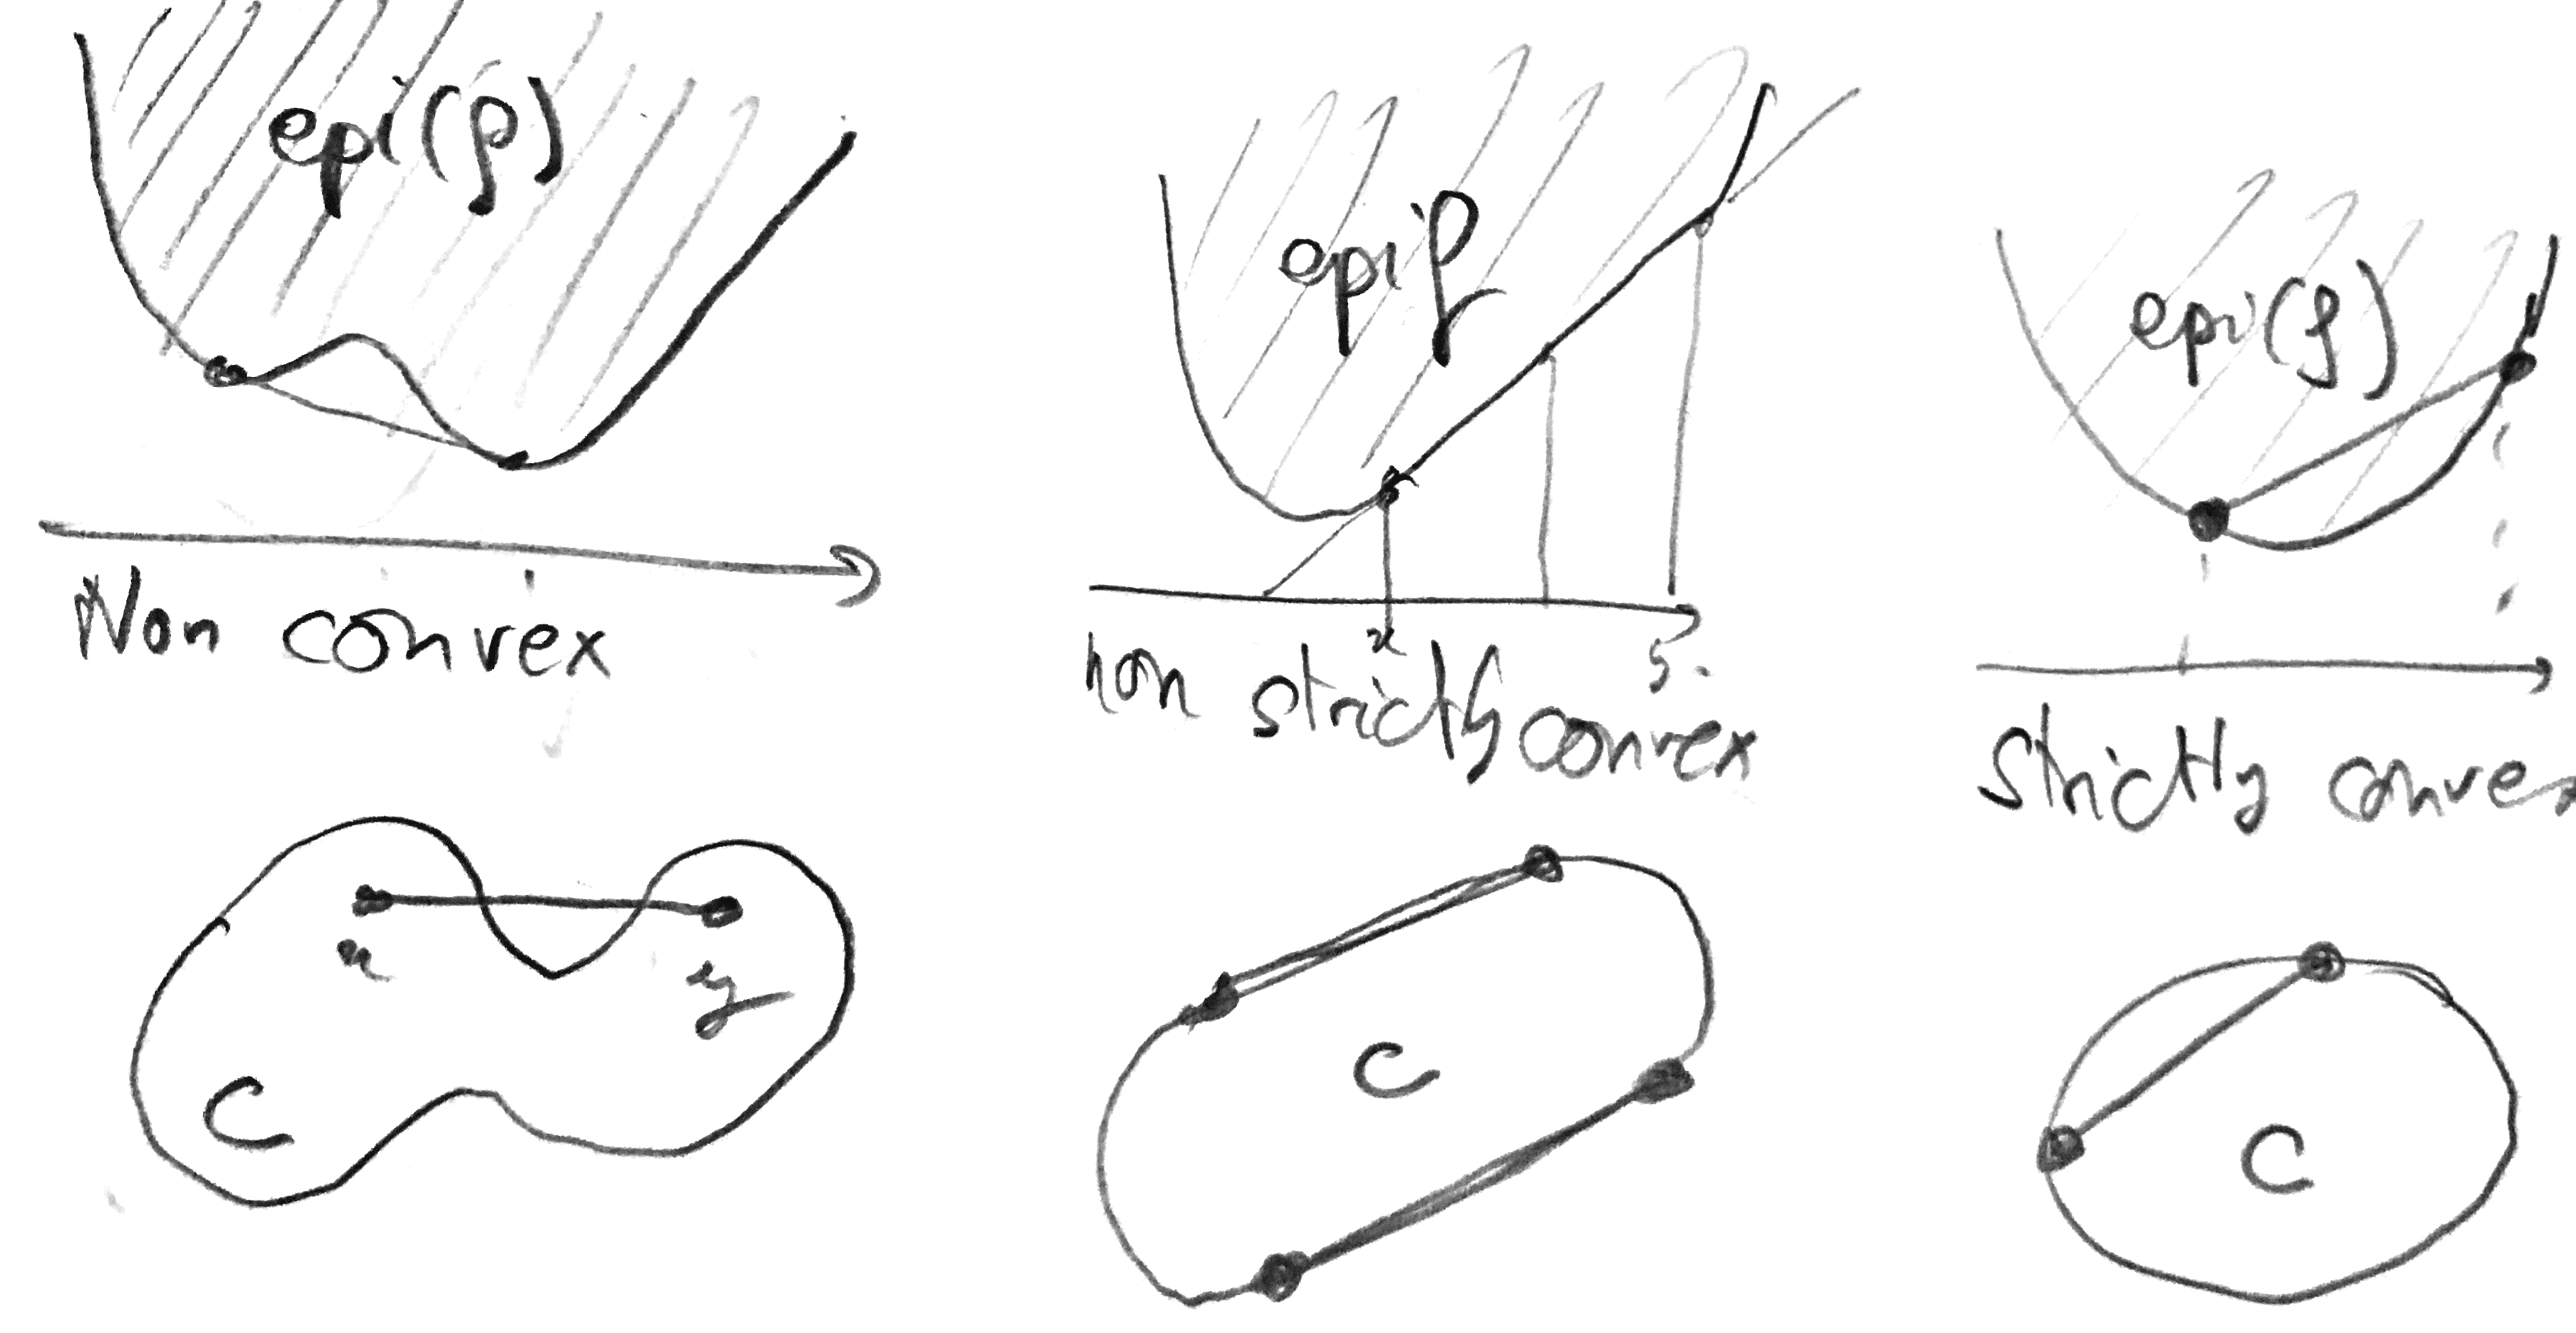
\includegraphics[width=.6\linewidth]{convexity/convex-examples}
%%
\caption{\label{fig-convex-examples}
Convexity and strict convexity for function and sets.}
\end{figure}




In the remaining part of this chapter, we consider convex function $f$ which are proper, i.e. such that $\dom(f) \neq \emptyset$, and that should be lower-semi-continuous (lsc), i.e. such that for all $x \in \Hh$, 
\eq{
	\lim\inf_{y \rightarrow x} f(y)  \geq f(x). 
}
It is equivalent to $\epi(f)$ being a closed convex set.
%
We denote $\Ga_0(\Hh)$ the set of proper convex lsc functions.

%%%%%%%%%%%%%%%%%%%%%%%%%%%%%%%%%%%%%%%%%%%%%%%%%%%%%%%%%%%%%%%%%%%%%%%%%%%%%%%%%%
\subsection{First Order Conditions}

%%%
\paragraph{Existence of minimizers.}

Before looking at first optimality conditions, one has to check that there exists minimizers, which is implied by the l.s.c. property and coercivity.

\begin{prop}
	If $f$ is l.s.c. and coercive (i.e. $f(x)\rightarrow +\infty$ as $x \rightarrow +\infty$), then there exists a minimizer $x^\star$ of $f$. 
\end{prop}

\begin{proof}
Since $f$ is coercive, it is bounded from bellow, one can consider a minimizing sequence $(x_n)_n$ such that $f(x_n) \rightarrow \min f$. 
%
Since $f$ is l.s.c., this implies that the sub-level set of $f$ are closed, and coercivity imply they are bounded, hence compact. One can thus extract from $(x_n)_n$ a converging sub-sequence $(x_{n(p)})_p$, $x_{n(p)} \rightarrow x^\star$. Lower semi-continuity implies that $\min f = \lim_p f(x_{n(p)}) \geq f(x^\star)$, and hence $x^\star$ is a minimizer.
\end{proof}

This existence proof is often called the ``direct method of calculus of variation''.
%
Note that if the function $f$ is in $\Ga_0(\Hh)$, then the set of minimizer $\argmin f$ is a closed convex set, and all local minimizers (i.e. minimizer of the function restricted to an open ball) are global one. If it is furthermore strictly convex, then there is a single minimizer. 

%%%
\paragraph{Sub-differential.}

The sub-differential at $x$ of such a $f$ is defined as
\eq{
	\partial f(x) \eqdef \enscond{u \in \Hh^*}{ \forall y, f(y) \geq f(x) + \dotp{u}{y-x} }.
}
We denote here $\Hh^* = \RR^N$ the set of ``dual'' vector. Although in finite dimensional Euclidean space, this distinction is not needed, it helps to distinguish primal from dual vectors, and recall that the duality pairing implicitly used depends on the choice of an inner product.
%
The sub-differential $\partial f(x)$ is thus the set of ``slopes'' $u$ of tangent affine planes $f(x) + \dotp{u}{z-x}$ that fits bellow the graph of $f$. 


\wrapf{convexity/subdifferential}{The subdifferential}
Note that $f$ being differentiable at $x$ is equivalent to the sub-differential being reduced to a singleton (equal to the gradient vector)
\eq{
	\partial f(x) = \{ \nabla f(x) \}. 
}
Informally, the ``size'' of $\partial f(x)$ controls how smooth $f$ is at $x$.

Note that one can have $\partial f(x) = \emptyset$, for instance if $x \notin \dom(f)$. Note also that one can still have $x \in \dom(f)$ and $\partial f(x) = \emptyset$, for instance take $f(x)=-\sqrt{1-x^2} + \iota_{[-1,1]}(x)$ at $x=\pm 1$. 

Since $\partial f(x) \subset \Hh^*$ is an intersection of half space, it is a closed convex set.
%  and it is non-empty if and only if $x \in \dom(f)$.
%
The operator $\partial f : \Hh \mapsto 2^{\Hh^*}$ is thus ``set-valued'', and we often denote this as $\partial f : \Hh \hookrightarrow \Hh^*$.

\begin{rem}[Maximally monotone operator]
The operator $\partial f$ is particular instance of so-called monotone operator, since one can check that $U=\partial f$ satisfies 
\eq{
	\foralls (u,v) \in U(x) \times U(y), \quad
		\dotp{y-x}{v-u} \geq 0. 
}
In the 1-D setting, being monotone is the same as being an increasing map.
%
Sub-differential can also be shown to be maximally monotone, in the sense that such an operator is not striclty included in the graph of another monotone operator. 
%
Note that there exists monotone maps which are not subdifferential, for instance $(x,y) \mapsto (-y,x)$. 
% 
Much of the theory of convex analysis and convex optimization can be extended to deal with arbitrary maximally monotone-maps in place of subdifferential, but we will not pursue this here.
\end{rem}

A prototypical example is the absolute value $f(x)=|\cdot|$, and writing conveniently $\partial f(x) = \partial |\cdot|(x)$, one verifies that
\eq{
	\partial |\cdot|(x) = 
	\choice{
		-1 \qifq x < 0, \\
		+1 \qifq x > 0, \\
		{[-1,1]} \qifq x=0.
	}
}

\begin{figure}
\centering
%%
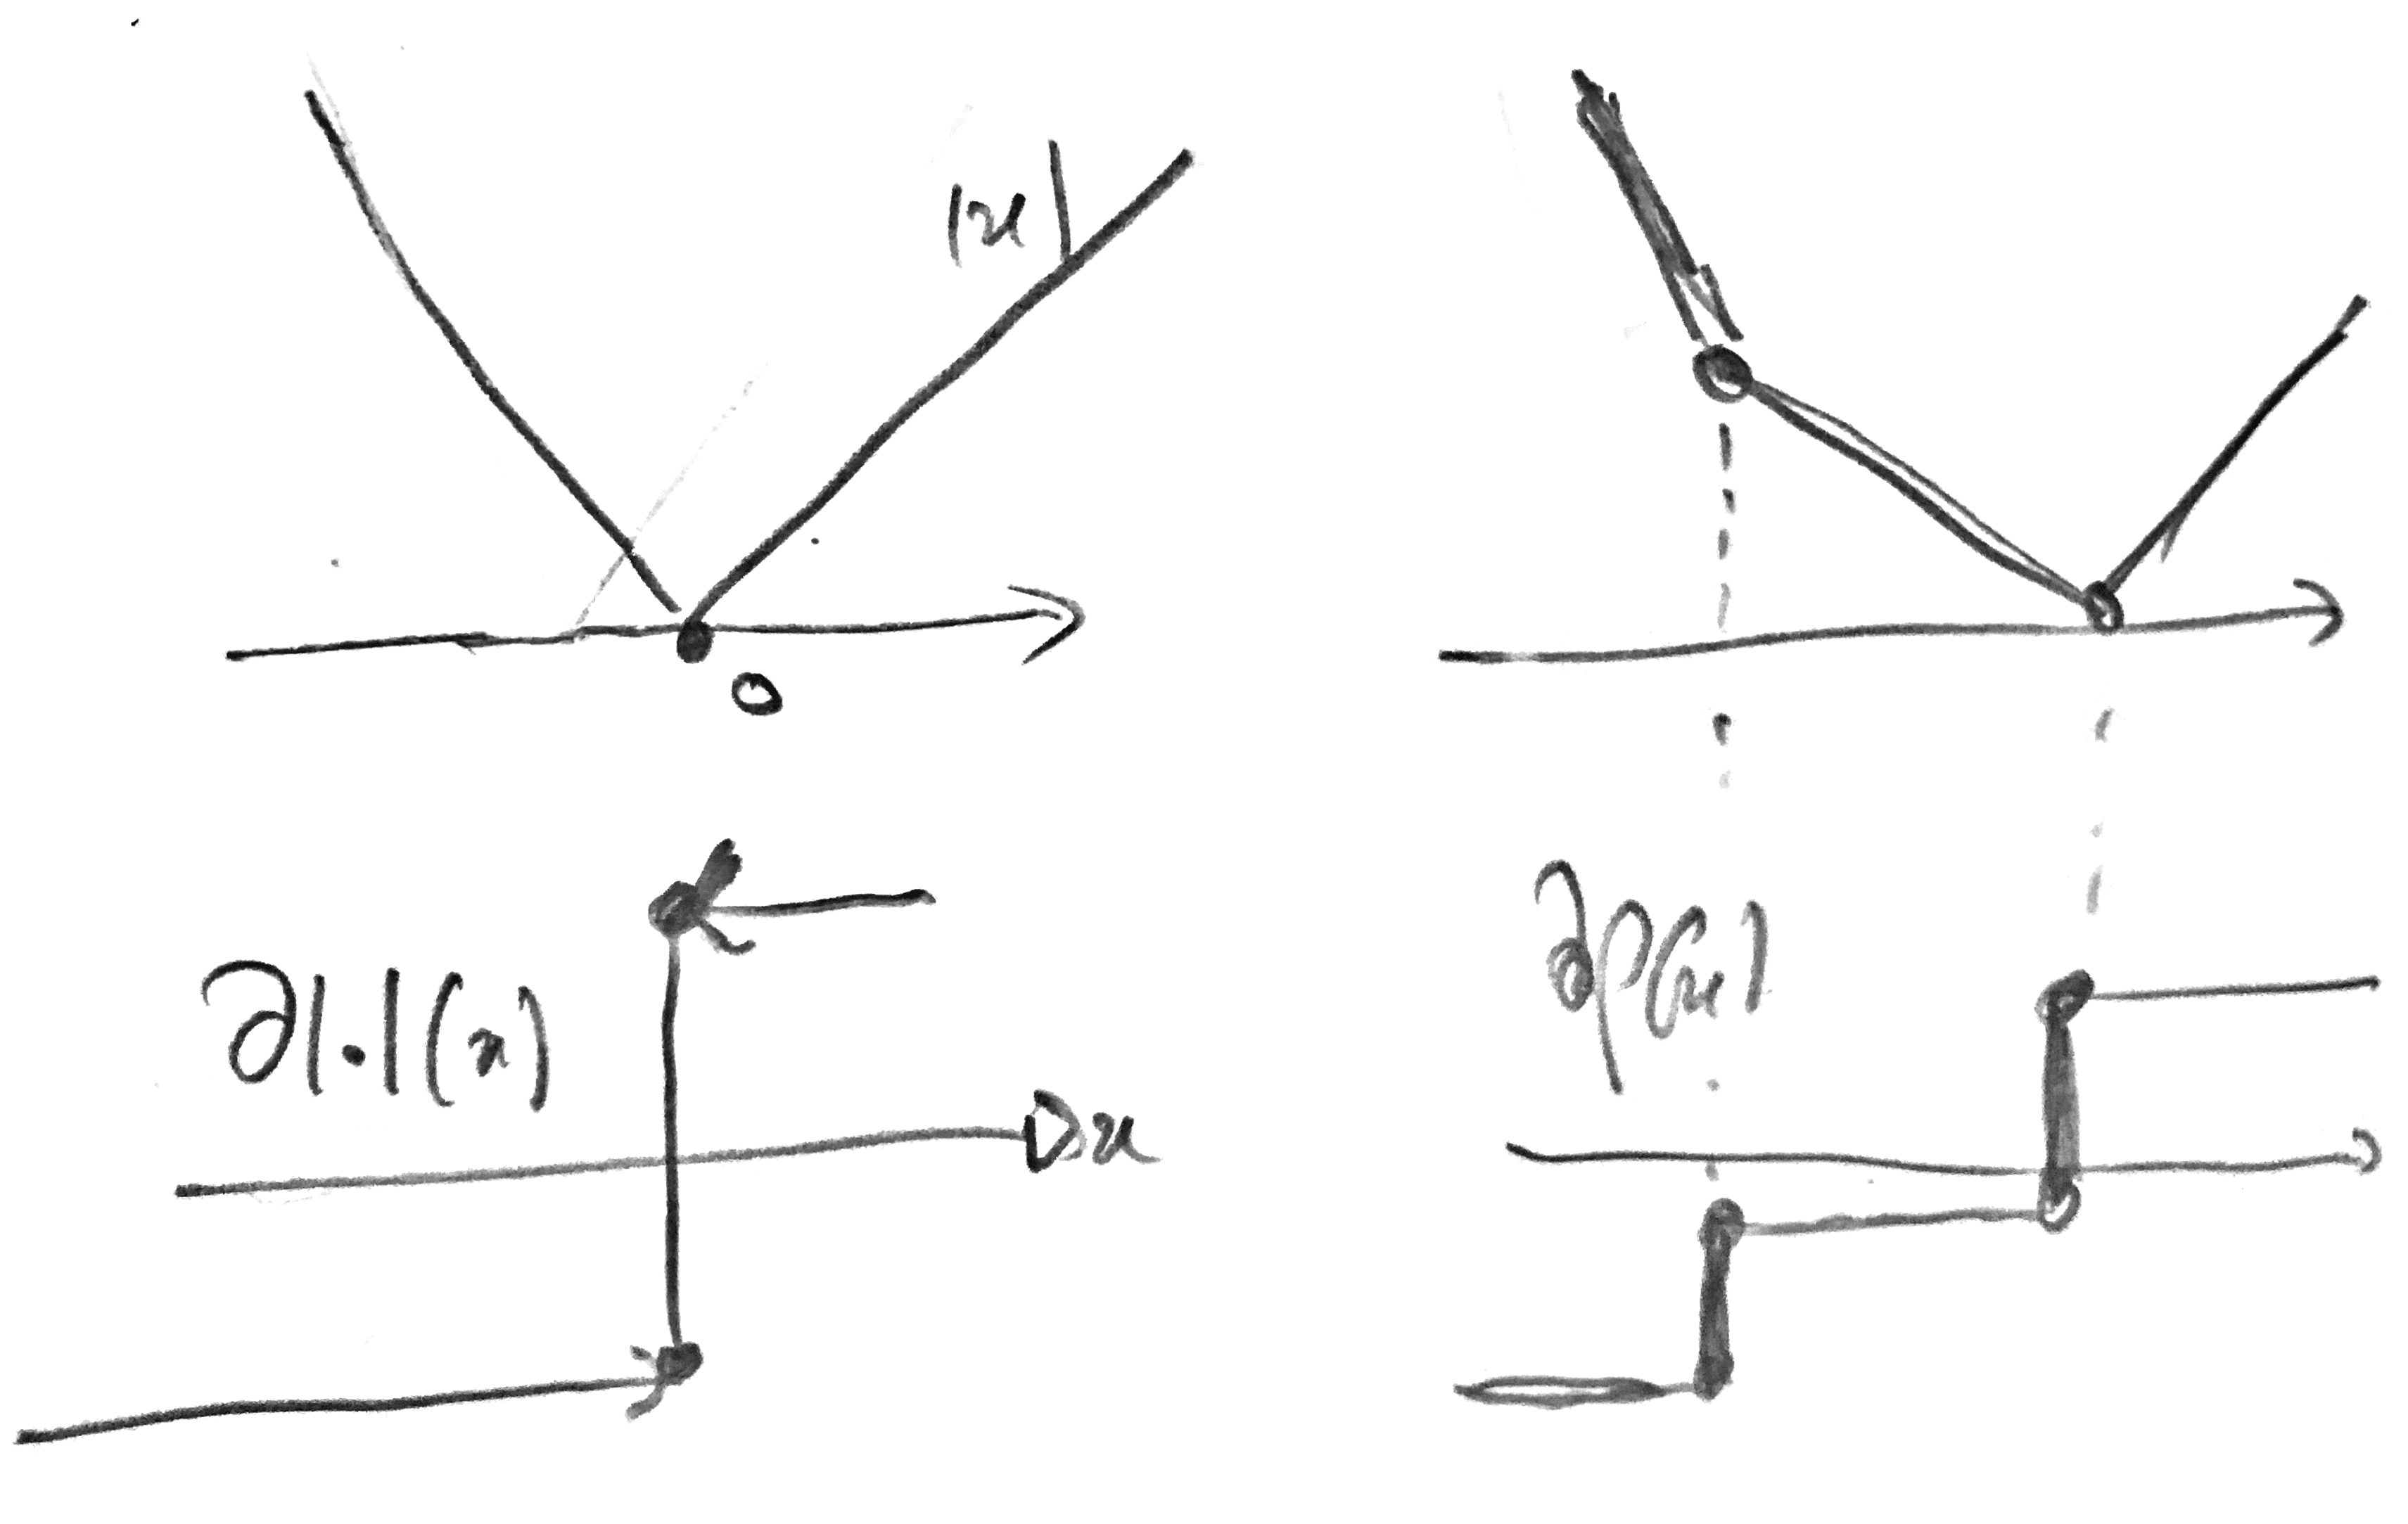
\includegraphics[width=.6\linewidth]{convexity/subdiff-l1}
%%
\caption{\label{fig-subdiff-l1}
Subdifferential of the absolute value and a piecewise affine convex function.}
\end{figure}







%%%
\paragraph{First Order Conditions.}

The subdifferential is crucial for this simple but extremely important proposition.

\begin{prop}
	$x^\star$ is a minimizer of $f$ is and only if $0 \in \partial f(x^\star)$.
\end{prop}
\begin{proof}
	One has
	\eq{
		x^\star \in \argmin f
		\quad\Leftrightarrow\quad
		\pa{ \forall y, f(x^\star) \leq f(y) + \dotp{0}{x^\star-y} }
		\quad\Leftrightarrow\quad
		0 \in \partial f(x^\star).
	}
\end{proof}

%%%
\paragraph{Sub-differential calculus.}

There is a large set of calculus rules that allows to simplify the computation of sub-differentials. For decomposable function $f(x_1,\ldots,x_K)=\sum_{k=1}^K f_k(x_k)$, the sub-differential is the product of the sub-differentials
\eq{
	\partial f(x_1,\ldots,x_K) = \partial f_1(x_1) \times \ldots \times \partial f_K(x_K).
}
This can be used to compute the sub-differential of the $\ell^1$ norm $\norm{x}_1=\sum_{k=1}^N |x_k|$
\eq{
	\partial \norm{\cdot}_1(x) = \prod_{k=1}^N \partial |\cdot|(x_k)
}
which is thus an hyper rectangle. This means that, denoting $I = \supp(x)$, one has $u \in \partial \norm{\cdot}_1(x)$ is equivalent to 
\eq{
	u_I = \sign(x_I)
	\qandq
	\norm{u_{I^c}}_\infty \leq 1.
}

A tricky problem is to compute the sub-differential of the sum of two functions. If one of the two function is continuous at $x$ (i.e. it has a finite value), then 
\eq{
	\partial (f+g)(x) = \partial f(x) \oplus \partial g(x) = \enscond{u+v}{(u,v) \in \partial f(x) \times \partial g(x)}
}
where $\oplus$ thus denotes the Minkowski sum. For instance, if $f$ is differentiable at $x$, then 
\eq{
	\partial (f+g)(x) = \nabla f(x) + \partial g(x) = \enscond{\nabla f(x) + v }{ v \in \partial g(x) }.
}
Positive linear scaling is simple to handle
\eq{
	\foralls \la \in \RR_+, \quad
	\partial (\la f)(x) = \la (\partial f(x)). 
}

The chain rule for sub-differential is difficult since in general composition does not work so-well with convexity. 
%
The only simple case is composition with linear functions, which preserves convexity. Denoting $A \in \RR^{P \times N}$ and $f \in \Ga_0(\RR^P)$, one has that $f \circ A \in \Ga_0(\RR^N)$ and
\eq{
	\partial (f \circ A)(x) = A^* (\partial f)(Ax) \eqdef \enscond{A^* u}{ u \in \partial f(Ax) }. 
}


%%%
\paragraph{Normal cone.}


The sud-differential of an indicator function is a convex cone, the so-called normal cone to the constraint
\eq{
	\foralls x \in \Cc, \quad \partial \iota_\Cc(x) = \Nn_\Cc(x) \eqdef \enscond{ v }{ \foralls z \in \Cc, \dotp{z-x}{v} \leq 0 }.
}
Note that for $x \notin \Cc$, $\partial  \iota_\Cc(x) = \emptyset$.
%
For an affine space $\Cc = a+\Vv$ where $\Vv \subset \Hh$ is a linear space, then $\Nn_\Cc(x)=\Vv^\bot$ is the usual orthogonal for linear spaces. If $x \in \inter(\Cc)$ is in the interior of $\Cc$, then $\Nn_\Cc(x)=\{0\}$. In some sense, the more non-regular the boundary of $\Cc$ is at $x$, the larger is the normal cone. 






\wrapf{convexity/normal-cone}{Normal cones}
The normal cone is a way to express first order condition for constrained problem
\eq{
	\umin{x \in \Cc} f(x)
}
which reads, if $f$ is continuous
\eq{
	0 \in \partial f(x) + \partial \iota_{\Cc}(x)
	\quad\Leftrightarrow\quad
	\exists \xi \in \partial f(x), - \xi \in \Nn_\Cc(x)
	\quad\Leftrightarrow\quad
	\partial f(x) \cap (-\Nn_\Cc(x)) \neq \emptyset.
}
If $f$ is differentiable, it reads $-\nabla f(x) \in \Nn_\Cc(x)$.



%%%%%%%%%%%%%%%%%%%%%%%%%%%%%%%%%%%%%%%%%%%%%%%%%%%%%%%%%%%%%%%%%%%%%%%%%%%%%%%%%%
%%%%%%%%%%%%%%%%%%%%%%%%%%%%%%%%%%%%%%%%%%%%%%%%%%%%%%%%%%%%%%%%%%%%%%%%%%%%%%%%%%
%%%%%%%%%%%%%%%%%%%%%%%%%%%%%%%%%%%%%%%%%%%%%%%%%%%%%%%%%%%%%%%%%%%%%%%%%%%%%%%%%%
\section{Convex Duality}
\label{sec-cvx-duality}

Duality is associated to a particular formulation of the optimization problem, so that for instance making change of variables results in a different duality. 

%%%%%%%%%%%%%%%%%%%%%%%%%%%%%%%%%%%%%%%%%%%%%%%%
\subsection{Lagrange Duality}

We consider a minimization of the form
\eql{\label{eq-lagrange-primal}
	p^\star = \umin{x \in \RR^N} \enscond{ f(x) }{ Ax=y \qandq g(x) \leq 0 }
}
for a continuous convex functions $f : \Hh \rightarrow 0$, a matrix $A \in \RR^{P \times N}$ and a function $g : \Hh \rightarrow \RR^Q$ such that each of its coordinates $g_i : \Hh \rightarrow \RR$ are continuous and convex.  
%
Note that it is always the case that equality in convex program corresponds to affine ones. 
%
One can always write a convex minimization problem with positivity constraints in the form~\eqref{eq-lagrange-primal}, although there exists infinite way of doing so (each one giving a different duality formula). 

Here we have assumed for simplicity that $f$ is continuous, i.e. $\dom(f)=\RR^N$.
%
The following exposition can be generalized to $\dom(f)$ being arbitrary, but this is more technical. For the sake of simplicity, we thus assume all the constraint defining the domain are encoded in $Ax=y$ and $g(x) \leq 0$


Note that it is possible to generalized the previous Lagrange duality results by replacing ``$x \geq 0$'' by ``$X \succeq 0$'' where $X$ is a matrix (and in fact even more generally using convex cones). 

We use the following fact
\eq{
	\usup{u \in \RR^P} \dotp{r}{u} = \choice{
		0 \qifq r=0, \\
		+\infty \qifq r \neq 0, 
	}
	\qandq
	\usup{v \in \RR_+^Q} \dotp{s}{v} = \choice{
		0 \qifq s \leq 0, \\
		+\infty \text{ otherwise}, 
	}
}
to encode the constraints $r=Ax-y=0$ and $s=g(x) \leq 0$.

One can represent the constraints appearing in~\eqref{eq-lagrange-primal} conveniently using a maximization over so-called Lagrange multipliers
\eq{
	p^\star = \uinf{x} \umax{u \in \RR^P, v \in \RR_+^Q } \Ll(x,u,v) \eqdef f(x) + \dotp{Ax-y}{u} + \dotp{g(x)}{v} .
}

It is tempting to inverse the inf and the sup, and study 
\begin{align}\label{eq-lagrange-dual}
	d^\star = \usup{(u,v) \in \RR^P \times \RR_+^Q } F(u,v) &\eqdef \uinf{x}  f(x) + \dotp{Ax-y}{u} + \dotp{g(x)}{v}.
\end{align}
One remarks that $F$ is a concave function (as being the minimum of linear forms), and this ``dual'' problem is thus a maximization of a concave function. 


The following proposition is the so-called weak duality, which assert that values of the dual problems always lower bounds values of the primal one

\begin{prop}
	One always has, for all $(u,v) \in \RR^P \times \RR_+^Q$, % for $x$ such that $Ax=y, g(x) \leq 0$ and 
	\eq{
		F(u,v) \leq p^\star \qarrq d^\star \leq p^\star.
	}
\end{prop}
\begin{proof}
	Since $g(x) \leq 0 $ and $v \geq 0$, one has $\dotp{g(x)}{v} \leq 0$, and since $Ax=y$, one has $\dotp{Ax-y}{u}=0$, so that 
	\eq{
		\Ll(x,u,v) \leq f(x) \qarrq F(u,v) = \uinf{x} \Ll(x,u,v) \leq \uinf{x} f(x) = p^\star.
	}
\end{proof}

The following fundamental theorem, more difficult to prove, gives a sufficient condition (so-called qualification of the constraints) such that one actually has equality.

\begin{thm}\label{thm-strong-duality}
	If 
	\eql{\label{eq-slater} 
		\exists x_0 \in \RR^N, \quad
			Ax_0=y \qandq g(x_0)<0, 
	}
	then $p^\star=d^\star$. Furthermore, $x^\star$ and $(u^\star,v^\star)$ are  solutions of respectively~\eqref{eq-lagrange-primal} and~\eqref{eq-lagrange-dual} if and only if
	\begin{align}
		\label{eq-lagr-dual-1}  & Ax^\star=y, \quad g(x^\star) \leq 0, \quad u^\star \geq 0 \\
		\label{eq-lagr-dual-2} 0 &\in \partial f(x^\star) + A^*u^\star + \sum_i v_i^\star \partial g_i(x^\star) \\
		\label{eq-lagr-dual-3}  \foralls i, \quad & u_i^\star g_i(x^\star) = 0
	\end{align}
\end{thm}

The existence of such an $x_0$ is called ``constraint qualification'', and as written here, this corresponds to the so-called ``Slater'' qualification condition (many other weaker sufficient conditions exist). 

Condition~\eqref{eq-lagr-dual-1} is simply the primal and dual constraints. 
%
Condition~\eqref{eq-lagr-dual-2} is the first order condition for the minimization of $\Ll(x,u,v)$ over $x$.
%
Condition~\eqref{eq-lagr-dual-3} is the first order condition for the maximization of $\Ll(x,u,v)$ over $(u,v)$.
%
These three conditions are often referred to as ``Karush-Kuhn-Tucker'' (KKT) conditions, and under a constraint qualification condition, they are necessary and sufficient condition for optimality. 


The last condition $u_i^\star g_i(x^\star) = 0$ (so called ``complementary slackness'') states that if $g_i(x^\star)<0$ (the constraints is not saturated) then $u_i=0$, and also that if $u_i>0$ then $g_i(x^\star)=0$.

Note that it is possible to weaken the hypotheses of this theorem, for the linear constraints of the form $g_i(x) = \dotp{x}{h_i} - c_i \leq 0$, by replacing the $g_i(x_0)<0$ by the weaker condition $\dotp{x_0}{h_i} \leq c_i$.

One can generalize this theorem to the setting where $\dom(f)$ is not equal to $\RR^N$ (i.e. it is not continuous, and thus integrates extra constraint beside the $\leq$). In this case, one has to add the extra constraint $x_0 \in \relint(\dom(f))$.
	
Theorem~\ref{thm-strong-duality} generalizes the necessary conditions provided by Lagrange multipliers for equality constrained optimization. The setting is both more complex because one can deal with inequalities that might be saturated (so this introduce positivity constraints on the multipliers $v$) but also simpler because of convexity (which thus gives also necessary conditions).

As a simple example, we now derive the dual for a simple linear projection problem. A more complicated computation is carried over in Section~\ref{sec-duality-lasso} for the Lasso. We consider
\begin{align*}
	p^\star = \umin{Ax=y} \frac{1}{2}\norm{x-z}^2 &= \umin{x} \umax{u} \frac{1}{2}\norm{x-z}^2 + \dotp{Ax-y}{u}
	= \umax{u} F(u) = \umin{x} \frac{1}{2}\norm{x-z}^2 + \dotp{Ax-y}{u}, 
\end{align*}
where we used the fact that strong duality holds because only linear constraints are involved.
%
For each $u$, the optimal $x$ satisfies $x-z+A^*u$, i.e. $x=z-A^*u$, so that 
\eq{
	F(u) = \frac{1}{2}\norm{A^*u}^2 + \dotp{A(z-A^*u)-y}{u} = -\frac{1}{2}\norm{A^*u}^2 + \dotp{u}{Az-y}.
}
Weak duality states $p^\star \geq F(u)$ for any $u$, and $p^\star = F(u^\star)$ where the optimal $u^\star$ satisfies $AA^*u = Az-y$. If $y \in \Im(A)$, then such a $u^\star$ exists and can be chosen as $u^\star = u=(AA^*)^{-1} (Az -y)$, and the (unique) primal solution reads 
\eql{\label{eq-proj-aff}
	x^\star = \Proj_{A\cdot=y}(z) (\Id-A^+A)z - A^+y.
}

%%%%%%%%%%%%%%%%%%%%%%%%%%%%%%%%%%%%%%%%%%%%%%%%
\subsection{Legendre-Fenchel Transform}

In order to simplify and accelerate computation involving Lagrange duality, it is very convenient to introduce a particular transformation of convex functions the Legendre-Fenchel transform. In some sense, it is the canonical ``isomorphisms'' (pairing) between convex functions. In spirit, is plays a similar role for convex function as the Fourier transform for signal or images. 

For $f \in \Ga_0(\Hh)$, we define its Legendre-Fenchel transform as
\eql{\label{eq-fenchel-transf}
	f^*(u) \eqdef \usup{x} \dotp{x}{u} - f(x).
}
Being the maximum of affine functional, one obtains that $f^*$ is itself a convex function, and that in fact $f^\star \in \Ga_0(\Hh^*)$. One can prove the following fundamental bi-duality result.

\begin{thm}
One has
\eq{
	\foralls f \in \Ga_0(\Hh), \quad (f^{*})^* = f. 
}
\end{thm}

In fact, $f^*$ is convex even in the case where $f$ is not, and $f^{**}$ is the convex envelop of $f$ (i.e. the largest convex function smaller than $f$). \todo{drawing}


One has the following basic property relating the sub-differentials of $f$ and $f^*$.

\begin{prop}
One has $\partial f^* = (\partial f)^{-1}$, where the inverse of a set valued map is defined in~\eqref{eq-inv-setvalued}, and 
\eq{
	\foralls (x,y), \quad \dotp{x}{y} \leq f(x) + f^*(y)
	\qandq
	\dotp{x}{y} = f(x) + f^*(y) 
	\quad\Leftrightarrow\quad x \in \partial f^*(y)
	\quad\Leftrightarrow\quad y \in \partial f(x).
}
\end{prop}

\begin{prop}\label{prop-dual-lp}
	For $1/p+1/q=1$, 
	\eq{
		( \iota_{\norm{\cdot}_p \leq 1} )^* = \norm{\cdot}_q
		\qandq
		( \norm{\cdot}_q  )^* =  \iota_{\norm{\cdot}_p \leq 1}
	}
\end{prop}


Let us now give some example of Legendre transform. 

\begin{prop}\label{eq-example-legendre}
	For $f(x)=\frac{1}{2}\dotp{Ax}{x} - \dotp{b}{x}$ with $A$ inversible, then $f^*(u) = \frac{1}{2}\dotp{A^{-1} u}{u} - \frac{1}{2}\dotp{A^{-1} b}{b}$.
	In particular, for $f=\norm{\cdot}^2/2$, then $f^*=f$. 
	One has\todo{check}
	\eq{
		f(\cdot-z)^* = f + \dotp{z}{\cdot}, \quad
		(f + \dotp{z}{\cdot})^* = f(\cdot-z), \quad
		(\la f)^* = \la f^*(\cdot/\la).		
	}
\end{prop}
\begin{proof}
	One has $f^*(u) = \dotp{Ax^\star}{x^\star} - \dotp{b}{x^\star}$ where $x^\star$ solves
	\eq{
		u = Ax^\star-b \qarrq
		x^\star = A^{-1} u + A^{-1} b.
	}
	Hence
	\eq{
		f^*(u)  = \frac{1}{2}\dotp{A A^{-1} ( u +  b )}{A^{-1}( u +  b)} - \dotp{b}{A^{-1} (u + b)}
			= \frac{1}{2}\dotp{A^{-1} u}{u} 
			- \frac{1}{2}\dotp{A^{-1} b}{b}
	}
	
\end{proof}

%%%%
\paragraph{Legendre transform and smoothness.}

While the Fourier transform is a pairing between smoothness and decay (see Section~\ref{}), the Legendre-Fenchel is really a pairing between smoothness and strong convexity. This can be intuitively seen by the fact that the Legendre-Fenchel inverts the sub-differentials~\eqref{} and hence when the functions involved are $\Cc^2$, it inverse the Hessians 
\eq{
	\partial^2 f(x) = ( \partial^2 f^*(y) )^{-1} \quad \text{at} \quad y = \nabla f(x).
}
This relation between Hessian can be seen as implying the exchange of strong convexity and uniform bound on the Hessian, as detailed in Proposition~\ref{prop-smooth-strong}.

\begin{prop}
	One has
	\eq{
		\nabla f \text{ is $L$-Lipschitz } 
		\quad\Longleftrightarrow\quad
		\nabla f^* \text{ is $\mu$-strongly convex.} 
	}
\end{prop}

This results suggests a way to smooth any function $f$. Instead of doing a convolution, one can use the infimal convolution
\eq{
	(f \otimes g)(x) \eqdef \usup{ y+y'=x } f(y) + g(y').
}
One can check that if $(f,g)$ are convex, so is $f \otimes g$, and that the Legendre transform actually exchanges sum and inf-convolution
\eq{
	( f+g )^* = f \otimes g 
	\qandq 
	( f \otimes g )^* = f + g.
}
The Moreau-Yosida regularization of $f$ is corresponds to a $\mu$-strict-convexification of $f^*$, i.e.
\eql{\label{eq-moreau-yosida}
	f_\mu \eqdef f \otimes (\frac{1}{2\mu}\norm{\cdot}^2) = ( f^* + \frac{\mu}{2}\norm{\cdot}^2 )^*.
}
Since $f^* + \frac{\mu}{2}\norm{\cdot}^2$ is at least $\mu$-strongly convex, then $f_\mu$ as a $1/\mu$-Lipchitz gradient.

As an example, the Moreau-Yosida regularization of the absolute value reads
\eq{
	(|\cdot|_\mu)(x) = 
	\choice{
		\frac{1}{2\mu}x^2 \qifq |x| \leq \mu, \\
		|x|-\frac{\mu}{2} \qifq |x|>\mu.
	}
}
This should be compared with the regularization $\sqrt{x^2+\mu^2}$ (which is above the curve) that we used previously. \todo{add drawing}



%%%%%%%%%%%%%%%%%%%%%%%%%%%%%%%%%%%%%%%%%%%%%%%%
\subsection{Fenchel-Rockafellar Duality}

%It is possible to express the Lagrange duality in term of Fenchel transform. Indeed for instance, re-write~\eqref{eq-lagrange-primal} as
%\eq{
%	\umin{(x,z) \in \RR^N} \enscond{ f(x) }{ Ax=y, x=z \qandq g(z) \leq 0 }
%}
%and then form the Lagrange dual
%\begin{align*}
%	 \umax{u \in \RR^P, v \RR_-^Q, w \in \RR^N } &\umin{x,z}  f(x) + \dotp{Ax-y}{u} + \dotp{x-z}{w} + \dotp{g(z)}{v} \\
%	 \umax{u \in \RR^P, v \RR_-^Q, w \in \RR^N } &\umin{x} f(x) + \dotp{x}{A^*u+w} + \sum_i \umin{z} - \dotp{z}{w} + g_i(z) {v_i} \\
%\end{align*}

Very often the Lagrange dual can be expressed using the conjugate of the function $f$. We give here a particularly important example, which is often called Fenchel-Rockafellar Duality. 

We consider the following structured minimization problem
\eql{\label{eq-fench-rock-basicpb}
	p^\star = \uinf{x} f(x) + g(Ax).	
}
Re-writing it as 
\eq{
	\uinf{y=Ax} f(x) + g(y), 
}
we can form the primal-dual problem
\eq{
	\uinf{(x,y)} \usup{u} f(x) + g(y) + \dotp{Ax-y}{u}. 
}
If sufficient condition on the domain of $(f,g)$ holds (such as those stated in Theorem~\ref{}), one one can exchange the min and the max and obtains the dual problem
\begin{align}\label{eq-deriv-rock-fench}
	d^\star &= \usup{u} \umin{(x,y)} f(x) + g(y) + \dotp{Ax-y}{u} \\
	&= \usup{u} \pa{ \umin{x} \dotp{x}{A^* u} + f(x) } + \pa{ \umin{y} -\dotp{y}{u} + g(y) } 
\end{align}
which leads to the celebrated Fenchel-Rockafellar, which we summarize together with qualification sufficient condition ensuring strong duality.

\begin{thm}[Fenchel-Rockafellar]\label{thm-fenchel-Rockafellar}
If 
\eql{\label{eq-qualif-fenchrock}
	0 \in \relint( \dom(g) ) - A \relint( \dom(f) )
}
the one has the following strong duality
\begin{align}\label{eq-fenchel-Rockafellar}
	\uinf{x} f(x) + g(Ax) &= \uinf{x} \usup{u} \Ll(x,u) 
	= \usup{u} \uinf{x}\Ll(x,u)  
	= \usup{u} - f^*(-A^*u) - g^*(u)
\end{align}
\eq{
	\qwhereq  \Ll(x,u)  \eqdef f(x) + \dotp{Ax}{u}  - g^*(u).
}
Furthermore one has that $(x^\star,u^\star)$ is a pair of optimal primal-dual solutions if and only if
\eql{\label{eq-primal-dual}
	-A^* u^\star \in \partial f(x^\star)  
	\qandq
	A x^\star \in  \partial g^*(u^\star).
}
\end{thm}

Condition~\eqref{eq-qualif-fenchrock} is the constraint qualification ensuring that one can inverse the inf and the sup in~\eqref{eq-fenchel-Rockafellar}. It can be recovered from Slater's qualification condition~\eqref{eq-slater} when deriving the dual problem as in~\eqref{eq-deriv-rock-fench}.
%
The primal-dual relations~\eqref{eq-primal-dual} are the first order condition along the $x$ and the $u$ variables in minimization and maximization of $\Ll$. They are sometimes summarised in ``matrix'' form 
\eq{
	0 \in 
	\begin{pmatrix}
		\partial f & A^* \\
		-A & \partial g^*
	\end{pmatrix}
	\begin{pmatrix}
		x^\star \\
		u^\star
	\end{pmatrix}.
}